\documentclass{beamer}
%
\mode<presentation>
{
  \usetheme{CambridgeUS}

  \setbeamercovered{transparent}
}
\usefonttheme[onlylarge]{structurebold}
\usepackage[polish]{babel}
\usepackage[utf8]{inputenc}
%\setbeameroption{show notes}
%
%\usepackage{times}
%\usepackage[T1]{fontenc}
\usepackage{ae}
\usepackage{tikz}
\usepackage{ulem}
\usepackage{color}
%
\newcommand{\marked}[1]{{\bf #1}}
\newcommand{\markerr}[1]{\textcolor{red}{#1}}
%
\title{Tagery morfosyntaktyczne dla języka polskiego}
%
\author{Łukasz Kobyliński \and Witold Kieraś}
%
\institute[IPI PAN]{%
     Instytut Podstaw Informatyki Polskiej Akademii Nauk\\
     ul. Jana Kazimierza 5, 01-248 Warszawa, Poland}
%
\date{7.12.2015}
%
\setbeamercolor{block title}{use=structure,fg=white,bg=purple!75!black}
\setbeamercolor{block body}{use=structure,fg=black,bg=white!20!white}
%
\setbeamertemplate{section page}
{
    \begin{centering}
    \begin{beamercolorbox}[sep=12pt,center]{part title}
    \usebeamerfont{section title}\insertsection\par
    \end{beamercolorbox}
    \end{centering}
}
%
\begin{document}
\begin{frame}
  \titlepage
\end{frame}

\begin{frame}{Wprowadzenie}
\structure{Cele prezentacji}
\begin{itemize}
  \item podsumowanie obecnego stanu narzędzi do tagowania morfosyntaktycznego w języku polskim,
  \item porównanie dokładności i wykorzystywanych algorytmów z narzędziami dla innych języków europejskich,
  \item analiza jakościowa wyników działania poszczególnych tagerów,
  \item przegląd problemów, które nie zostały zaadresowane przez istniejące tagery,
  \item rekomendacje dotyczące dalszych kroków.
\end{itemize}
\end{frame}

\begin{frame}
\frametitle{Plan}
\tableofcontents
\end{frame}

\section{Tagery języka polskiego -- przegląd rozwiązań}
\frame{\sectionpage}

\begin{frame}{Czym jest tagowanie -- przypomnienie}
  \structure{Segment (token)} -- wyraz lub jego fragment, znak interpunkcyjny, ciąg cyfr
lub symboli. Segmenty są ciągłe oraz rozłączne.
  \vspace{0.5cm}

  \structure{Znacznik morfosyntaktycnzy (tag)} -- symbol, który można przypisać segmentowi, określający jego własności morfologiczno-składniowe.
  \vspace{0.5cm}

  \structure{Znakowanie morfosyntaktyczne (tagowanie)} -- zadanie przypisania ciągowi segmentów ciągu znaczników morfosyntaktycznych.
  \vspace{1cm}

  \structure{Segmentacja} $\Rightarrow$ \structure{Analiza morfosyntaktyczna} $\Rightarrow$ \structure{Ujednoznacznianie morfosyntaktyczne}
\end{frame}

\begin{frame}{Pełny stos przetwarzania}
  \begin{columns}[c]
    \column{.5\textwidth}
    \begin{center}
  TAGOWANIE
  Podział na tokeny - Toki
  Analiza morfosyntaktyczna - Maca + Morfeusz
  Ujednoznacznianie morfosyntaktyczne
\end{center}
\column{.5\textwidth}
\begin{center}
  UCZENIE
  Ponowna analiza morfosyntaktyczna otagowanego tekstu - Toki + Maca + Morfeusz + synchronizacja
  Uczenie modelu statystycznego na podstawie wzorca
\end{center}
\end{columns}
\end{frame}

\begin{frame}{Tagery morfostynaktyczne dla języka polskiego}
\structure{Tagery historyczne}
\begin{itemize}
\item tager Łukasza Dębowskiego,
\item TaKIPI.
\end{itemize}
\end{frame}

\begin{frame}{Tagery morfostynaktyczne dla języka polskiego}
\structure{Tagery uwzględniające tagset NKJP}
\begin{itemize}
\item Pantera [Acedański 2010] -- adaptacja algorytmu Brilla do języków bogatych morfologicznie, takich jak polski,
\item WMBT [Radziszewski and Śniatowski 2011] -- tager oparty na uczeniu pamięciowym, rozbudowany o wielowarstwowość dla uwzględnienia wielu atrybutów znakowania w języku polskim,
\item Concraft [Waszczuk 2012] -- tager warstwowy, oparty na Conditional Random Fields (CRF); wyniki dezambiguacji morfosyntaktycznej przekazywane są z jednej warstwy do drugiej,
\item WCRFT [Radziszewski 2013] -- również oparty na CRF; osobne modele wykorzystywane są do dezambiguacji poszczególnych atrybutów opisu morfosyntaktycznego,
\end{itemize}
\end{frame}

\begin{frame}{Tagery morfostynaktyczne dla języka polskiego}
\structure{Modele dla tagerów zaimplementowanych dla innych języków}
\begin{itemize}
\item TnT Tagger
\item OpenNLP
\end{itemize}
\end{frame}

\begin{frame}{Przenośność i łatwość wykorzystania}
  \begin{itemize}
    \item \structure{Concraft} instalowany i uruchamiany z wykorzystaniem Haskell Platform, która dostępna jest pod wszystkie główne systemy operacyjne,
    \item \structure{WCRFT, Pantera} -- wymagają kompilacji, proces kompilacji dostosowany do środowiska Linuksowego,
    \item \structure{WMBT} -- Python.
  \end{itemize}
  \vspace{1cm}

  \structure{Concraft, WCRFT, WMBT} -- silnie zależą od stosu Corpus2 / Toki / Maca, których kompilacja pod Windows jest możliwa, ale nietrywialna (Visual Studio).
\end{frame}

\section{Tagery języka polskiego -- analiza ilościowa}
\frame{\sectionpage}

\begin{frame}{Metoda ewaluacji}
\structure{Miara jakości znakowania}
\begin{itemize}
\item ze względu na możliwość wystąpienia różnic w segmentacji pomiędzy wynikiem znakowania, a złotym standardem, wykorzystujemy dolne ograniczenie trafności (\emph{accuracy lower bound}, $Acc_{lower}$) do oceny dokładności tagerów,
\item miara ta karze wszelkie zmiany segmentacyjne w stosunku do złotego standardu i traktuje takie tokeny jako sklasyfikowane błędnie,
\item token traktowany jest jako oznakowany prawidłowo, jeśli zbiór jego interpretacji ma niepuste przecięcie ze zbiorem interpretacji zwracanych przez tager,
\item niezależne sprawdzamy dokładność dla znanych ($Acc^K_{lower}$) i nieznanych słów ($Acc^U_{lower}$), aby ocenić skuteczność ew. modułów odgadywania.
\end{itemize}
\end{frame}

\begin{frame}{Ewaluacja pojedynczych tagerów}
\structure{Eksperymenty na milionowym podkorpusie Narodowego Korpusu Języka Polskiego, ver. 1.1, 10-krotna walidacja krzyżowa.}
\begin{center}
\begin{tabular}{lcccc} \hline
n & Tager 		& $Acc_{lower}$	& $Acc^K_{lower}$	& $Acc^U_{lower}$	\\ \hline
1 & Pantera   & 88.95\%   & 91.22\% & 15.19\% \\
2 & WMBT	 	& 90.33\%		& 91.26\%	& 60.25\%	\\
3 & WCRFT	 	& 90.76\%		& 91.92\%	& 53.18\%	\\
4 & Concraft	& 91.07\%		& 92.06\%	& 58.81\%	\\
\end{tabular}
\end{center}
\begin{itemize}
\item $Acc_{lower}$ -- łączna dokładność,
\item $Acc^K_{lower}$ -- dokładność dla znanych słów,
\item $Acc^U_{lower}$ -- dokładność dla słów nieznanych.
\end{itemize}
\end{frame}

\begin{frame}{Analiza rezultatu działania tagerów}
\structure{Porównanie wyników}
\begin{itemize}
\item Wszystkie zwracają prawidłowy tag: \marked{82,78\%} \\
{\footnotesize \underline{unikam} fin:sg:pri:imperf\\
fin:sg:pri:imperf+ fin:sg:pri:imperf+ fin:sg:pri:imperf+ fin:sg:pri:imperf+}
\item Większość zwraca prawidłowy tag: \marked{7,95\%} \\
{\footnotesize \underline{kapitalistów} subst:pl:gen:m1 \\
subst:pl:gen:m1+ subst:pl:gen:m1+ subst:pl:gen:m1+ subst:pl:acc:m1-}
\item Równowaga w głosowaniu: \marked{2,71\%} \\
{\footnotesize \underline{powolny} adj:sg:nom:m3:pos \\
adj:sg:nom:m3:pos+ adj:sg:nom:m3:pos+ adj:sg:acc:m3:pos- adj:sg:acc:m3:pos-}
\item Prawidłowy tag w mniejszości: \marked{2,38\%} \\
{\footnotesize \underline{twarzy} subst:sg:loc:f subst:sg:gen:f- subst:sg:gen:f- subst:sg:gen:f- subst:sg:loc:f+}
\item Wszystkie się mylą: \marked{4.18\%} \\
{\footnotesize \underline{biurka} subst:pl:nom:n subst:pl:acc:n- subst:pl:acc:n- subst:sg:gen:n- subst:pl:acc:n- \\
(Peggy) \underline{McCreary} subst:sg:nom:f \\
subst:sg:gen:f- subst:sg:gen:n- subst:sg:nom:n- subst:sg:acc:m1-}
\end{itemize}
\end{frame}

\begin{frame}{Podział na klasy gramatyczne}
\begin{center}
\begin{tabular}{llllll}
 &  & \multicolumn{4}{c}{$Acc_{lower}$ (\%)} \\
klasa & liczność & PANTERA & WMBT & WCRFT & Concraft \\
\hline
subst & 331570 & 85,21 & 86,25 & 87,36 & 88,29 \\
interp & 223542 & 99,63 & 99,97 & 99,97 & 99,97 \\
adj & 128703 & 76,53 & 81,10 & 81,56 & 82,52 \\
prep & 115818 & 97,04 & 97,28 & 97,54 & 98,05 \\
qub & 68079 & 92,98 & 93,82 & 92,91 & 92,92 \\
fin & 59458 & 98,64 & 98,70 & 98,81 & 98,94 \\
praet & 53326 & 90,90 & 88,96 & 89,80 & 89,69 \\
conj & 44840 & 95,17 & 95,41 & 94,61 & 93,96 \\
adv & 42750 & 95,31 & 95,59 & 95,29 & 94,77 \\
inf & 19213 & 98,91 & 99,20 & 99,09 & 99,14 \\
comp & 17842 & 97,26 & 97,29 & 96,84 & 96,88 \\
num & 16160 & 33,40 & 56,40 & 60,32 & 55,99 \\
\end{tabular}
\end{center}
\end{frame}

\begin{frame}{Problem niejednoznaczności segmentacji}
  \structure{Na czym polega problem?}\\
  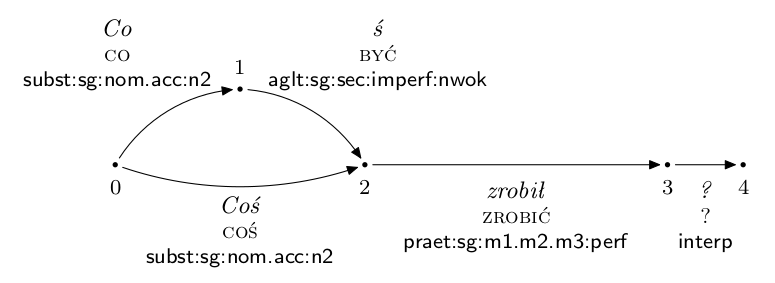
\includegraphics[width=\textwidth]{img/segm_amb1.png}
\end{frame}

\begin{frame}{Problem niejednoznaczności segmentacji}
  \structure{Jak często występują niejednoznaczności?}\\
  Korpus NKJP 1M, Morfeusz 1 SGJP:\\
  645 wystąpień na 1 095 118 segmentów (0.0589\%)
  \begin{columns}[c]
    \column{.3\textwidth}
    \begin{center}
      \footnotesize
      \begin{tabular}{l|r}
      kiedyś & 234 / \markerr{1} \\
      gdzieś & 172 / \markerr{1} \\
      miałem & 99 / \markerr{98} \\
      udziałem & 40 / 0 \\
      musiałem & 28 / \markerr{28} \\
      sms-a & 6 / 0 \\
      działam & 6 / 0\\
      doń & 5 / \markerr{4} \\
      tyłem & 4 / 0 \\
      pis-em & 4 / 0 \\
      podziałem & 3 / 0 \\
      piekłem & 3 / 0 \\
      czekałem & 3 / \markerr{3} \\
      jadłem & 3 / \markerr{3} \\
      \end{tabular}
    \end{center}
    \column{.3\textwidth}
    \begin{center}
      \footnotesize
      \begin{tabular}{l|r}
        pis-owi & 3 \\
        winnym & 2 \\
        prl-em & 2 \\
        wyłom & 2 \\
        rozdziałem & 2 \\
        hiv-em & 2 \\
        pit-ów & 2 \\
        działem & 1 \\
        rop-em & 1 \\
        tir-a & 1 \\
        kor-owcy & 1 \\
        urm-em & 1 \\
        kor-em & 1 \\
        dj-a & 1 \\
      \end{tabular}
    \end{center}
    \column{.3\textwidth}
    \begin{center}
      \footnotesize
      \begin{tabular}{l|r}
        ipn-em & 1 \\
        sms-ów & 1 \\
        pgr-ach & 1 \\
        zus-em & 1 \\
        vat-em & 1 \\
        siadłem & 1 \\
        msz-ów & 1 \\
        zoz-ów & 1 \\
        mosir-em & 1 \\
        vip-om & 1 \\
        msz-ecie & 1 \\
        zoz-owi & 1 \\
        czemuś & 1 \\
      \end{tabular}
    \end{center}
  \end{columns}
\end{frame}

\begin{frame}{Problem niejednoznaczności segmentacji}
  \structure{Jak często występują niejednoznaczności?}\\
  Próbka 100M NKJP, Morfeusz 1 SGJP:\\
  40 354 wystąpień na 101 052 527 segmentów (0.0399\%)
  \begin{columns}[c]
    \column{.3\textwidth}
    \begin{center}
      \footnotesize
      \begin{tabular}{l|r}
        kiedyś & 12751 \\
        miałem & 8350 \\
        gdzieś & 6171 \\
        udziałem & 4988 \\
        musiałem & 2173 \\
        czekałem & 537 \\
        tyłem & 523 \\
        doń & 414 \\
        podziałem & 411 \\
        sms-a & 357 \\
        vip-ów & 305 \\
        winnym & 256 \\
        sms-ów & 207 \\
        jadłem & 199 \\
      \end{tabular}
    \end{center}
    \column{.3\textwidth}
    \begin{center}
      \footnotesize
      \begin{tabular}{l|r}
        czemuś & 171 \\
        działam & 153 \\
        działem & 151 \\
        piekłem & 130 \\
        zus-em & 95 \\
        sms-em & 95 \\
        tir-ów & 93 \\
        zoz-ów & 86 \\
        tir-a & 85 \\
        zus-owi & 82 \\
        azs-em & 81 \\
        vat-em & 76 \\
        rozdziałem & 76 \\
        wyłom & 65 \\
      \end{tabular}
    \end{center}
    \column{.3\textwidth}
    \begin{center}
      \footnotesize
      \begin{tabular}{l|r}
        pit-ów & 65 \\
        Łks-em & 60 \\
        pis-em & 44 \\
        siadłem & 43 \\
        skok-i & 39 \\
        gks-em & 39 \\
        padłem & 36 \\
        pgr-ów & 30 \\
        vip-a & 30 \\
        pis-owi & 28 \\
        skok-ów & 24 \\
        pks-em & 24 \\
        dj-ów & 20 \\
        dj-e & 20 \\
      \end{tabular}
    \end{center}
  \end{columns}
\end{frame}

\begin{frame}{Problem niejednoznaczności segmentacji}
  \structure{Jak często występują niejednoznaczności?}\\
  Korpus NKJP 1M, Morfeusz 2:\\
  2583 wystąpień na 1 095 118 segmentów (0.2359\%)
  \begin{columns}[c]
    \column{.3\textwidth}
    \begin{center}
      \footnotesize
      \begin{tabular}{l|r}
        coś & 777 \\
        ktoś & 382 \\
        czym & 334 \\
        kiedyś & 234 \\
        gdzieś & 172 \\
        miałem & 99 \\
        czegoś & 97 \\
        kogoś & 82 \\
        czymś & 63 \\
        kimś & 42 \\
        gdybym & 40 \\
        udziałem & 40 \\
        żebym & 39 \\
        żebyś & 34 \\
      \end{tabular}
    \end{center}
    \column{.3\textwidth}
    \begin{center}
      \footnotesize
      \begin{tabular}{l|r}
        komuś & 31 \\
        gdybyśmy & 19 \\
        tom & 19 \\
        żebyśmy & 12 \\
        gdybyś & 7 \\
        działam & 6 \\
        jam & 5 \\
        doń & 5 \\
        oścież & 5 \\
        gdybyście & 4 \\
        tyłem & 4 \\
        musiałem & 3 \\
        podziałem & 3 \\
        piekłem & 3 \\
      \end{tabular}
    \end{center}
    \column{.3\textwidth}
    \begin{center}
      \footnotesize
      \begin{tabular}{l|r}
        czekałem & 3 \\
        jadłem & 3 \\
        rozdziałem & 2 \\
        wyłom & 2 \\
        bom & 2 \\
        żebyście & 2 \\
        coście & 1 \\
        czyżbyś & 1 \\
        czyżem & 1 \\
        siadłem & 1 \\
        czemuś & 1 \\
        działem & 1 \\
      \end{tabular}
    \end{center}
  \end{columns}
\end{frame}

\begin{frame}{Problem niejednoznaczności segmentacji}
  \structure{Możliwe rozwiązania: tagset pośredni}
  Pomysł od Adama Radziszewskiego
\end{frame}

\begin{frame}{Problem niejednoznaczności segmentacji}
  \structure{Możliwe rozwiązania: dostosowanie metody uczenia maszynowego do reprezentacji grafowej}
  Pomysł od Jakuba Waszczuka - CRFy
\end{frame}

\begin{frame}{Poziom pewności ujednoznaczniania morfosyntaktycznego}
  Concraft - marginals
\end{frame}

\begin{frame}{Problem lematyzacji}
\end{frame}

\section{Tagery morfostynaktyczne innych języków}
\frame{\sectionpage}

\begin{frame}{jakie rozwiązania są możliwe - jakie były na świecie}
  TODO
\end{frame}

\begin{frame}{jak wzrasta jakość tagowania wraz ze wzrostem ilości danych}
  TODO
\end{frame}

% ile razy się zgadzają, równowaga, przewaga, różne
% w ile procentach są wszystkie poprawne, większość poprawna, mniejszość poprawna, żaden nie jest poprawny

\section{Tagery języka polskiego -- analiza jakościowa}
\frame{\sectionpage}

\section{Dyskusja i rekomendacje}
\frame{\sectionpage}

\begin{frame}[fragile]{Różne tagsety dla języka polskiego?}
  \structure{Obecnie funkcjonują równolegle dwa tagsety języka polskiego}
  \begin{itemize}
    \item tagset NKJP, używany do anotacji korpusu, a także w większości innych zasobów językowych,
    \item tagset SGJP, używany w słowniku Morfologicznym i w Morfeuszu.
  \end{itemize}
  \vspace{0.5cm}

  Skutkuje to sytuacją, w której w sposób niejawny dokonywana jest ciągła konwersja pomiędzy tagsetami:
  \begin{columns}[c]
    \column{0.3\textwidth}
      \footnotesize
      \begin{verbatim}
        tagset_from=sgjp
        tagset_to=nkjp
        override=n1:n
        override=n2:n
        override=n3:n
        override=p1:m1
        override=p2:n
        override=p3:n
      \end{verbatim}
    \column{0.7\textwidth}
      \footnotesize
      \begin{verbatim}
        tagset_from=morfeusz2; tagset_to=nkjp
        override=dig:num; override=nie:conj
        override=romandig:num
        override=prefa:ign
        override=prefppas:ign
        override=prefs:ign; override=prefv:ign
        override=naj:ign; override=cond:ign
        override=substa:ign
      \end{verbatim}
    \end{columns}
\end{frame}

\begin{frame}{Struktura danych treningowych w NKJP1M}
  TODO
\end{frame}

\begin{frame}{Podziękowania}
  \structure{Podziękowania za sugestie i uwagi dla:}
  \begin{itemize}
    \item Adama Radziszewskiego
    \item Jakuba Waszczuka
    \item Szymona Acedańskiego
  \end{itemize}
\end{frame}

\begin{frame}{}
\begin{centering}
    \begin{beamercolorbox}[sep=12pt,center]{part title}
    \usebeamerfont{section title}Dziękujemy za uwagę!\par
    \end{beamercolorbox}
    \end{centering}
\end{frame}

\begin{frame}[allowframebreaks]
  \frametitle{Bibliografia}
  \begin{thebibliography}{10}
  \beamertemplatebookbibitems
  \bibitem[Acedański, 2010]{ace:2010}
Acedański, Szymon, 2010.
\newblock A morphosyntactic {B}rill tagger for inflectional languages.
\newblock In {\em Advances in Natural Language Processing\/}.
  \beamertemplatearticlebibitems
  \bibitem[Brill and Wu, 1998]{bri:wu:1998}
Brill, Eric and Jun Wu, 1998.
\newblock Classifier combination for improved lexical disambiguation.
\newblock In {\em Proceedings of the 17th international conference on
  Computational linguistics - Volume 1\/}, COLING '98. Stroudsburg, PA, USA:
  Association for Computational Linguistics.
  \beamertemplatearticlebibitems
  \bibitem[Śniatowski and Piasecki, 2012]{sni:pia:2012}
Śniatowski, Tomasz and Maciej Piasecki, 2012.
\newblock Combining {P}olish morphosyntactic taggers.
\newblock In Pascal Bouvry, Mieczysław~A. Kłopotek, Franck Leprévost,
  Małgorzata Marciniak, Agnieszka Mykowiecka, and Henryk Rybiński (eds.),
  {\em Security and Intelligent Information Systems\/}, volume 7053 of {\em
  LNCS\/}. Springer-Verlag.
  \beamertemplatearticlebibitems
  \bibitem[Radziszewski, 2013]{rad:2013}
Radziszewski, Adam, 2013.
\newblock A tiered {CRF} tagger for {P}olish.
\newblock In R.~Bembenik, {\L}.~Skonieczny, H.~Rybi\'{n}ski, M.~Kryszkiewicz,
  and M.~Niezg{\'o}dka (eds.), {\em Intelligent Tools for Building a Scientific
  Information Platform: Advanced Architectures and Solutions\/}. Springer
  Verlag.
  \beamertemplatearticlebibitems
  \bibitem[Radziszewski and Acedański, 2012]{rad:ace:2012}
Radziszewski, Adam and Szymon Acedański, 2012.
\newblock {T}aggers gonna tag: an argument against evaluating disambiguation
  capacities of morphosyntactic taggers.
\newblock In {\em Proceedings of TSD 2012\/}, LNCS. Springer-Verlag.
\beamertemplatearticlebibitems
\bibitem[Radziszewski and Śniatowski, 2011a]{rad:sni:2011}
Radziszewski, Adam and Tomasz Śniatowski, 2011a.
\newblock {A} {M}emory-{B}ased {T}agger for {P}olish.
\newblock In {\em Proceedings of the LTC 2011\/}.
\beamertemplatearticlebibitems
\bibitem[van Halteren et~al., 2001]{hal:dae:zav:2001}
van Halteren, Hans, Walter Daelemans, and Jakub Zavrel, 2001.
\newblock Improving accuracy in word class tagging through the combination of
  machine learning systems.
\newblock {\em Comput. Linguist.\/}, 27(2):199--229.
\beamertemplatearticlebibitems
\bibitem[Waszczuk, 2012]{wasz:12}
Waszczuk, Jakub, 2012.
\newblock Harnessing the {CRF} complexity with domain-specific constraints.
  {T}he case of morphosyntactic tagging of a highly inflected language.
\newblock In {\em Proceedings of the 24th International Conference on
  Computational Linguistics ({COLING}\,2012)\/}. Mumbai, India.
  \end{thebibliography}
\end{frame}

\end{document}
